\documentclass[a4paper,12pt]{article}
\usepackage{latexsym}
\usepackage{graphicx}
\usepackage{epsfig}
\usepackage{float}
\usepackage{natbib}
\usepackage{listings}
\graphicspath{{./}}
\DeclareGraphicsExtensions{.jpg}
\author{Howard Kinsman}
\title{Cosmology Essay: A review of Dark Matter and Dark Energy}
\begin{document}
\maketitle
\section{Introduction}
Many observations, and subequent cosmological theories, have found that approximately 95\% of the mass and energy in the universe is dark and invisible, the true nature of which is
largely unknown. The matter component is known as dark matter (DM) and the energy component dark energy (DE) This is a brief review of the history and current status of 
DM and DE.
\section{Dark Matter}
DM has a surprisingly long and interesting history. In 1933, the renowned astrophysicist, Fritz Zwicky published a paper on the velocity dispersion of galaxies within the Coma cluster. He found
that the velocity dispersion of galaxies within the cluster was so high that in order for the system to remain stable there must be some ``missing mass'' i.e. mass which
is not detectable optically. Further research in this area continued but it wasn't until the 1970s when astronomers began accurately measuring the rotation curves of spiral galaxies,
with the discovery of HI 21cm radio emission, that interest in this area became of great importance. HI 21cm radio emission is produced by neutral hydrogen during a change of energy
state. It has a very precise wavelength of 21cm.
Rotation curves are a measure of the orbital velocity of the stars and gas in a galaxy plotted as a function of distance from the galactic centre. According to
Keplerian laws rotation curves would be expected to decline with increasing radius however it was found that they remain flat i.e. constant, all the way out to the largest radii observed, 
both optically and with 21 cm. According to Newtonian gravity this implies that there must be some ``hidden mass'' within the galaxies exerting a gravitational effect on the system resulting
in these flat rotation curves. This ``hidden mass'' was termed dark matter.
\begin{figure}[H]
\centering
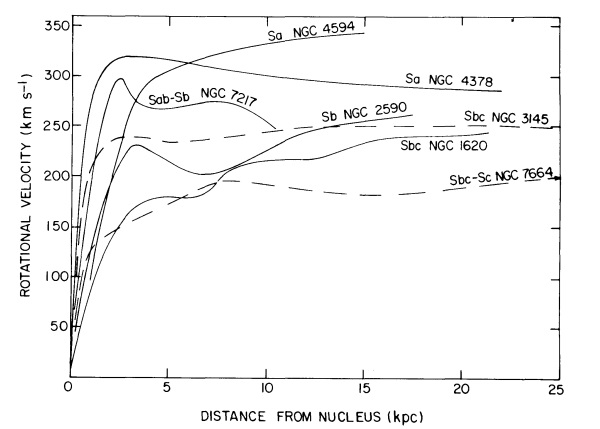
\includegraphics[width=.9\textwidth]{./rotationcurves.jpg}
\caption{Examples of flat galaxy rotation curves \citep{ruben}}
\label{fig:1}
\end{figure}

Apart from high velocity dispersions in galaxy clusters and flat rotation curves other evidence for DM includes gravitational lensing, hot gas in clusters, the Cosmic Microwave Background (CMB)
 and through computer modelling of the growth of 
large scale structure in the early universe (discussed later). Gravitational lensing occurs when light from distant galaxies behind a galaxy cluster is distorted due to the 
large gravitational pull of the cluster. This is known as strong lensing and is quite rare, however weak lensing also occurs where there is just a small distortion of the galaxies size
and shape. 
The mass of the galaxy cluster can be measured and compared to how much the light is expected to be bent by gravity. The results show that there must be far more mass in clusters 
than can be detected. Galaxy clusters when viewed in X-ray reveal huge amounts of hot gas which can only be explained by large amounts of DM which provide a potential gravitational well to hold the gas.
The CMB is the remnants of radiation from the early universe. Anisotropies in the CMB also reveal evidence for DM. Anisotropies are irregularities seen in the CMB which, after having been
thoroughly studied, reveal what woud be expected if thermal variations in a small space had grown to form the observable universe today.
Before decoupling from baryonic matter (i.e. ordinary matter comprised of 
mainly protons and neutrons), photons underwent oscillations that froze in at redshift $z\approx1100$. Decoupling refers to events in the early universe when different
particles fall out of thermal equilibrium with each other.
By studying the height of the peaks in these oscillations it has been 
found that the universe is comprised of approximately 5\% baryonic matter, 26\% dark matter
and the remainder dark energy (discussed later). Some authors \citep{freese} regard the evidence of DM from the CMB as ``irrefutable''.

Further evidence of DM, which has been described as ``direct empirical proof'' \citep{clowe}, has been found in observations of the Bullet cluster of galaxies. The Chandra X-ray observatory 
has detected the baryonic matter in the merger of two smaller clusters, whilst DM has been deduced from gravitational lensing, and they clearly show that are behaving differently.
At the collision point the baryonic matter has slowed down due to friction whilst the DM has passed through this point.
\begin{figure}[H]
\centering
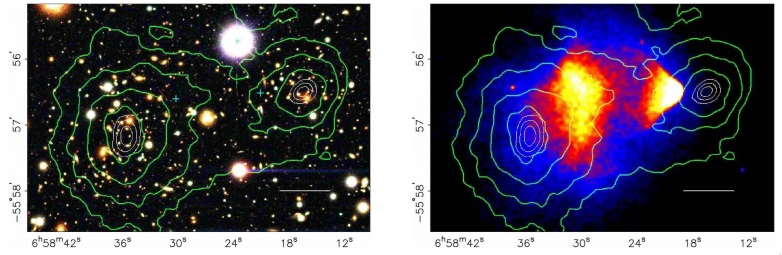
\includegraphics[width=.9\textwidth]{./bullet.jpg}
\caption{The bullet cluster: a) Optical view from Magellan telescope with plotted contours of mass distribution obtained from gravitational lensing.
b) Same contours but with Chandra X-ray data showing hot plasma. Most of the matter is lying in a different location to the hot plasma which has been slowed down by friction 
during the merger. \citep{clowe}}
\label{fig:2}
\end{figure}

With the growing evidence for the existence of DM, obvious questions to ask are ``What is it made of?'' and ``Is it baryonic?''. About twenty years ago it was suggested that dark matter is
comprised of objects such as faint stars, sub-stellar objects or stellar remnants. Collectively these came to be known as massive compact halo objects (MACHOs). However recent studies 
\citep{freese} have found that these objects couldn't account for all the DM in the universe. This then suggests that if DM exists it must be non-baryonic.

Particle physicists have postulated many possible candidates for non-baryonic DM particles. These include neutrinos, primordial black holes (PBHs), magnetic monopoles, neutalinos and photinos.
However, many of these have been effectively ruled out by research e.g. \cite{gaggero} who concluded that PBHs couldn't account for more than 20\% of DM in the universe.
Two of the most popular non-baryonic DM candidates currently are: Axions and Weakly Interacting Massive Particles (WIMPs). These are both hypothetical particles invented by particle 
physicists for other reasons than DM, which relieves cosmologists of having to invent new particles. Axions arise from a problem in quantum chromodynamics but have interesting 
consequences for cosmology as they are predicted to be stable over cosmological timescales \citep{bertone1} and could therefore theoretically constitute DM. WIMPs have been the source
of many theoretical studies of DM and are now considered to be the leading class of DM particles, partly because they are predicted to interact via gravity and have a large mass
compared to other particles.

There are currently four main approaches to discovering WIMPs. There are ongoing experiments, with ever increasing sensitivity, at CERN, using
the Large Hadron Collider. One of the goals of the two detectors, ATLAS and CMS, was specifically to try and discover the nature of DM. It has so far been unsuccessful in that respect.
There are also attempts to directly detect WIMPs in underground DM laboratories worldwide. So far there has been no confirmed detection of WIMPs. Indirect detection of WIMPs is also being
carried out in objects such as the galactic centre, galaxy clusters and dwarf galaxies i.e. objects with a predicted over-density of WIMPs. Again, there has been no confirmed detection.

An interesting fourth approach to the hunt for DM is to discover dark stars. It is predicted that the first stars to form in the early universe, at redshift $z\approx 10-50$, may have been 
comprised of mainly hydrogen and helium and yet were powered by DM heating rather than nuclear fusion. These are believed to have formed when the universe was much denser than now and 
consisted of high density DM halos. It is hoped that the James Webb Space Telescope will be able to detect dark stars and so enable us to study WIMPs in more detail.

With the advent of numerical simulations, models that involve DM have been extensively explored. Currently a very popular model of the evolution of structure in the universe is
the Lambda Cold Dark Matter ($\Lambda CDM$) model. $\Lambda$ here refers to the cosmological contant discussed in the DE section. 
Computer simulations have shown that if the DM particles are relativistic (``hot'') then, on small scales, density fluctuations are Silk damped, or
washed out, the random thermal motion of DM particles. This results in small scale structure fluctuations to be suppressed. However, if the DM particles are ``cold'' i.e. cold dark matter (CDM), then
they undergo a very different structure formation because they have a much smaller free-streaming length and can form low mass halos which can gradually build up into larger DM
structures. These DM structures provide a gravitational well that baryonic particles can fall into to form baryonic structure. This results in a bottom-up process of structure 
formation which is very different to the top-down sequence predicted for hot DM. These simulations have further convinced cosmologists that CDM comprised of WIMPs are the best
explanation for the growth of large scale structure in the universe. In fact, the $\Lambda CDM$ model agrees so well with observations that it is often regarded as the ``standard model
of cosmology''.

Even though the evidence for DM is growing, there has been no confirmed detection of DM or WIMPs and the theory of DM leads to a number of problems \citep{sellwood} which I don't
have space to detail here. This has led some cosmologists to believe that the Newtonian theory of gravity may need to be amended. One of these theories is called Modified Newtonian
Dynamics (MOND). It is a conceptually simple idea but it has some far-reaching consequences. The basic idea is that Newton's second law be amended from $F=ma$ to $F=ma^2/a_0$ in the
limit of very low accelerations ($a<<a_0\approx 1.2\times10^{-10}m/s^2$). This could then account for the observed motions of stars within galaxies without having to introduce
DM. MOND has been quite successful with explaining flat rotation curves but less successful with galaxy clusters. MOND, however, is not without its own problems particularly when it
comes to integrating MOND with general relativity (GR), explaining the growth of large scale structure, and explaining the first CMB acoustic peak.
It would appear that either the LHC, or any detection methods previously described, will eventually detect WIMPs and confirm the existence of DM and MOND will die out as a theory or, if
no detection of DM is forthcoming then the theory of MOND may well grow.

\section{Dark Energy}
Cosmic acceleration, and associated DE, is arguably one of the greatest unsolved problems in contemporary physics. DE actually has a longer history than DM. As Einstein was forming his 
field equations for general relativity he realised that this would result in a universe that would
gravitationally attract and therefore contract. He therefore introduced the cosmological constant to balance gravity and ensure a static universe. When observations by Hubble in 1929
revealed that the universe is expanding, Einstein referred to his failure to predict a dynamic universe has his biggest blunder. The cosmological constant therefore fell into disuse.
However, in 1980 Alan Guth and Alexei Starobinsky proposed the idea of cosmic inflation which involved an exponential expansion of the universe immediately after the Big Bang. The theory
of inflation involves a negative pressure field which creates a repulsive force. This idea is similar to DE, however even when inflation became widely accepted the 
cosmological constant was considered irrelevant. This changed however in 1998 when observations of supernovae revealed that the universal expansion is accelerating. This was the first
direct evidence of DE.

Type Ia supernovae occur when a white dwarf in a binary pair accretes enough mass so that it goes over the Chandrasekhar mass and triggers a supernova. The supernova therefore doesn't
depend on the mass of the white dwarf on the other star in the binary. Type Ia supernovae can be considered as standard candles and enable astronomers to obtain a luminosity distance.
To measure cosmic expansion the apparent magnitude of distant supernovae are compared to those of more local supernovae which are not affected by DE. The Supernova Cosmology Project
which carried out one of the surveys in 1998 found that, with a flat cosmology ($\Omega_{\Lambda}+\Omega_m=1$), that $\Omega_m=.28$ and so that $\Omega_{\Lambda}=.72$. $\Omega$ is the
density parameter and is defined as the ratio of the observed density to the critical density. $\Omega_m$ here is 
the proportion of matter in universe (DM and baryonic) whilst $\Omega_{\Lambda}$ represents the proportion of DE in universe. The deceleration parameter is calculated as follows:
\begin{equation}
\frac{1}{2}(\Omega_m-2\Omega_{\Lambda}+2\Omega_R) 
\end{equation}
This then results in a negative deceleration parameter indicating that the expansion of the universe is accelerating.
Since 1998 there have been many more supernova surveys and it is has become an active area of observational cosmology. All this supernova data indicates that the apparent luminosity
of Type Ia supernovae declines more rapidly with increasing redshift than would be expected if $\Omega_M=1$ and $\Omega_{\Lambda}=0$ i.e. an Einstein-de Sitter universe, or the 
luminosity distance is greater than expected. Of course, this data could be interpreted as being due to other effects such as dust or gas in the line of sight. More evidence is required.

Although it doesn't directly constrain DE, data obtained from CMB anisotropies does provide accurate figures for parameters that are needed in order to study DE. By measuring anisotropies 
within the CMB data, from WMAP and Planck satellites, accurate figures for $\Omega_B$ and $\Omega_{DM}$ have been obtained. 
\begin{figure}[H]
\centering
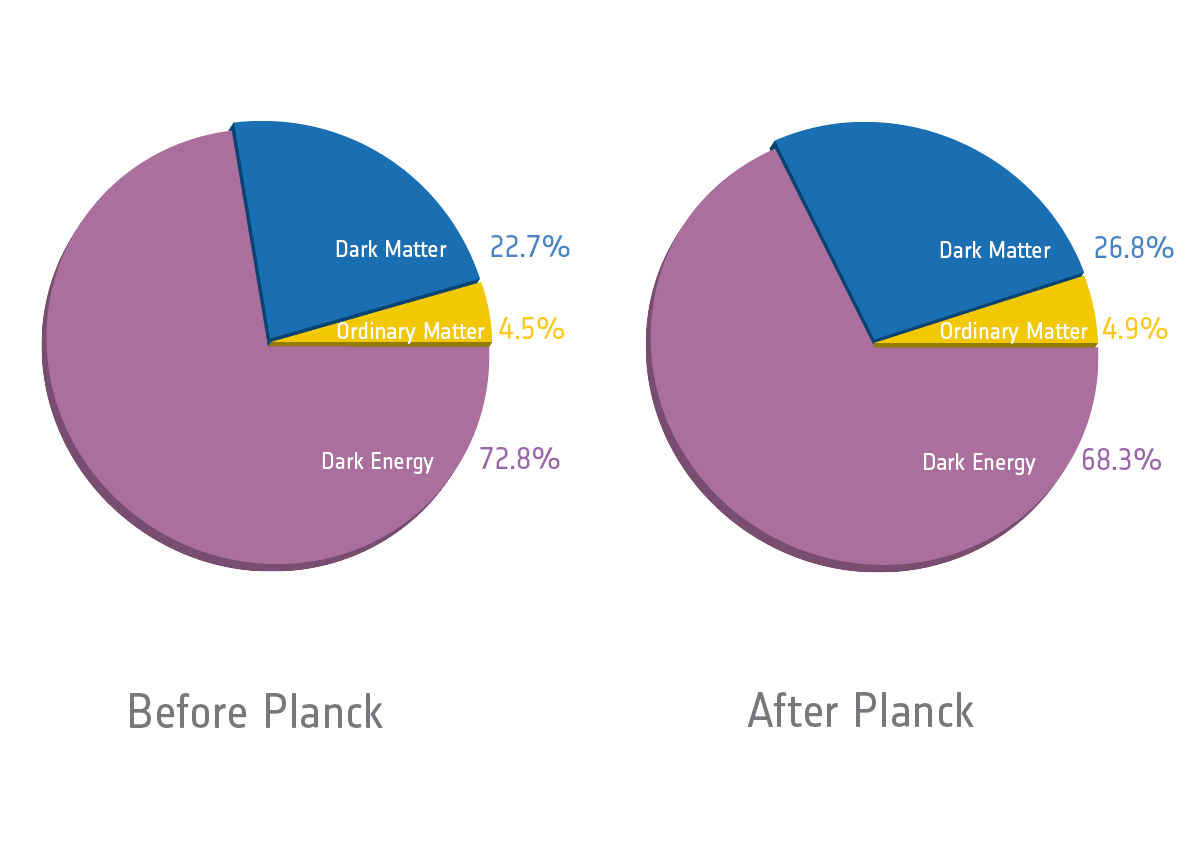
\includegraphics[width=.9\textwidth]{./planck2.jpg}
\caption{The Planck satellite helped provide accurate figures for cosmological parameters \citep{planck}}
\label{fig:3}
\end{figure}

Similarly, Baryonic Acoustic Oscillations (BAO) also
help the study of DE by constraining cosmological parameters. BAOs are regular and periodic fluctuations in the density of baryonic matter. They are measured by looking at large
scale structures in the universe through galaxy surveys. In a similar way that Type Ia supernovae
are standard candles, BAOs are standard rulers. By comparing the clustering of galaxies today (using redshift surveys like the Sloan Digital Sky Survey - SDSS) and comparing it with
data from CMB cosmologists have a way of measuring DE that is independent of the supernova method.

Unlike DM, where particle physicists and cosmologists have established theories as to what it may be comprised of, the nature of DE is completely unknown. DE is often referred to as
vacuum energy. According to quantum field theory a vacuum or empty space actually consists of transient fluctuations known as virtual particles. 
They do, however, have some properties in common with ``ordinary'' particles.
It has been suggested that these virtual particles may give
rise to DE. However, the density of virtual particles is about 120 times larger than the DE density. There is currently no explanation for this. The DE density is believed
to be $\approx10^{-27}kg/m^3$ which is low but it has such a profound effect on the universe because it fills all of empty space.

There are many theories for DE. However, the simplest one is that it is constant i.e. a cosmological constant. The cosmological constant has a negative pressure equal to
its energy density and so exerts a repulsive force causing the expansion of the universe to accelerate i.e. $P=-\rho$. The previously mentioned $\Lambda CDM$ model uses
this form of DE and is the currently preferred cosmological model. An important parameter in the study of DE is the equation of state parameter $\omega$. This comes from: 
\begin{equation}
P=\omega\rho c^2
\end{equation}
where P is pressue, $\rho$ is density, c is speed of light and $\omega$ is the equation of state parameter.
In the $\Lambda CDM$ model $\omega$ is assumed to be -1.

Another theory of DE is quintessence. In this theory, DE is assumed to be a scalar field and unlike the 
cosmological constant can vary in time and space. However, there is currently no evidence to support this theory.
It has been suggested that instead of vacuum energy, cosmic acceleration can be explained by a modified version of GR. Tests of GR within the solar system have proven the theory
to be accurate but it may be the case that GR breaks down on cosmological scales. However there currently is no viable theory of GR that can fully explain cosmic acceleration
without introducing some form of DE. However, this doesn't preclude a theory arising in the future as, for example, it wasn't until the advent of GR in 1915 that the precession
of Mercury's orbit could be fully explained.

The Dark Energy Survey (DES) was specifically created to probe DE. Using a wide-field camera on the 4m Blanco Telescope in Chile the project aims to catalogue 300 million
galaxies. The main goals of the survey are to characterise DE and DM and also to test alternative theories of gravity. The survey takes photometric redshifts of galaxies and
also carries out galaxy-galaxy weak lensing measurements i.e. where both the lenses and sources are galaxies. It is also carrying out a time domain survey of Type Ia supernovae.
Last year the project reported that they had further constrained $\Omega_m$ to be $=0.31\pm0.09$. The SDSS is also carrying out DE probes with the Extended Baryon Oscillation
Spectroscopic Survey (eBOSS). The main goals of eBOSS are to measure clustering on large scales and to measure BAOs. Other projects include Panoramic Survey Telescope and Rapid 
Response System (Pan-STARRS) and the Hobby-Eberly Telescope Dark Energy Experiment (HETDEX). 
One of the aims of Pan-STARRS was to constrain the equation of state parameter for DE ($\omega$) which was found to be $\omega=-1.14$ \citep{zheng}. The Hobby-Eberly Telescope 
has recently been upgraded for HETDEX and will probe DE through spectrographs of galaxies over the redshift $0<z<4$ and also analysing BAOs. The aim of HETDEX is to provide a
direct detection of DE at $z\approx3$ \citep{hill}.

A new and exciting development by the European Space Agency, which will further probe DE, will be the launch of Euclid which is expected to be in 2020. Euclid aims to find out
the nature the acceleration of the expansion of the universe and DE. It will measure shapes and redshifts of galaxies and also explore the large scale structure of the universe
by measuring the distribution of galaxy clusters. Euclid is a satellite equipped with a 1.2m telescope and three imaging and spectroscopic instruments working in optical and
near-infrared. It will be placed at the L2 Langrange point, a stable point in space, and is planned to operate for six years. The plan is cover 15000 square degrees of sky and
image one billion galaxies and take redshifts measurements of 100,000 galaxies \citep{amendola}. With this data Euclid will able to detail clustering of galaxies out to redshift
z=2 and out to redshift z=3 utilising weak lensing. Redshift measurements and weak lensing will also accompanied by measuring correlations with the CMB, obtaining galaxy cluster 
information, strong lensing and possibly even obtaining luminosity distance through supernovae Type Ia measurements.

DE may well have a profound effect on the final fate of the universe. Observations suggest that the expansion of the universe will continue to accelerate forever and so the 
universe will cool as it expands. Redshift will eventually stretch photons to undetectable wavelengths and galaxies will therefore appear to disappear. Star formation will cease 
as gas supply runs out. Stars will
eventually die out, one by one, leaving stellar remnants. Some theories even predict that stellar remnants will disappear due to proton decay leaving only black holes,
which themselves will eventually disappear due to Hawking radiation. Proton decay is a hypothetical form of radiactive decay in which protons decay into ligher particles. 
Hawking radiation is blackbody radiation believed to be emitted by black holes because of quantum
effects near the event horizon. This is often referred to as the heat death of the universe. It would seem that the ultimate fate of our universe could potentially be a very 
cold, dark void.

\begin{thebibliography}{1}
\bibitem[Abbott et al(2015)]{abbott}Abott, T., et al (Dark Energy Survey Collaboration), 2015, The Dark Energy Survey: more than dark energy - an overview, arXiv:1601.00329v3
\bibitem[Amendola et al(2016)]{amendola}Amendola, L., et al (Euclid Theory Working Group), 2016, Cosmology and Fundamental Physics with the Euclid Satellite, arXiv:1006.00180v1
\bibitem[Arun et al(2017)]{arun}Arun, K., Gudennavar, S., B., Sivaram, C., 2017, Dark Matter, Dark Energy, and Alternate Models: A Review, arXiv:1704.06155
\bibitem[Baldry(2016)]{baldry}Baldry, I., Cosmology lecture notes - MSc Astrophysics, 2016, Not in public domain
\bibitem[Bergstrom(2012)]{bergstrom}Bergstrom L., 2012,  Dark Matter Evidence, Particle Physics Candidates and Detection Methods, arXiv:1205.4882
\bibitem[Bertone et al(2004)]{bertone2}Bertone, G., Hooper, D., Silk, J., 2004, Particle Dark Matter: Evidence, Candidates and Constraints, arXiv:hep-ph/0404175v2
\bibitem[Bertone and Hooper(2016)]{bertone1}Bertone, G., Hooper, D., 2016, A History of Dark Matter, arXiv:1605.04909v2
\bibitem[Calmet and Kuntz(2017)]{calmet}Calmet, X., Kuntz, I., 2017, What is modified gravity and how to differentiate it from particle dark matter?, arXiv:1702.03832v2
\bibitem[Clowe et al(2006)]{clowe}Clowe, D., Bradac, M., Gonzalez, A., H., Markevitch, M., Randall, S., W., Jones, C., Zaritsky, D., 2006, A Direct Empirical Proof of the Existence of Dark Matter, arXiv:astro-ph/0608407v1
\bibitem[Cohen-Tannoudji(2015)]{cohen}Cohen-Tannoudji, G., 2015, The dark universe and quantum vacuum, arXiv:1507.00460
\bibitem[Fornengo(2017)]{forengo}Fornengo, N., 2017, Dark matter overview, arXiv:1701.00119v3
\bibitem[Freese(2017)]{freese}Freese, K., 2017, Status of dark matter in the universe, arXiv:1701.01840v1
\bibitem[Gaggero et al(2016)]{gaggero}Gaggero, D., Bertone, G., Calore, F., Connors, R., M., T., Lovell, M., Markoff, S., Storm E., 2016, Searching for Primodial Black Holes in the radio and X-ray sky, arXiv:1612.00457v1
\bibitem[He Zhang(2017)]{he}He, H., Zhang, Z., 2017, Direct Probe of Dark Energy through Gravitational Lensing Effect, arXiv:1701.03418v2
\bibitem[Hill et al(2008)]{hill}Hill,G., J., et al, 2008, The Hobby-Eberly Telescope Dark Energy Experiment (HETDEX): Description and Early Pilot Survey Results, arXiv:0806.0183v1
\bibitem[Li et al(2012)]{li}Li, M., Li., X.,Wang, S., Wang, Y., 2012, Dark Energy: a Brief Review, arXiv:1209.0922v1
\bibitem[Lisanti(2016)]{lisanti}Lisante M, 2016, Lectures on Dark Matter Physics, arXiv:1603.03797v2
\bibitem[Mortonson et al(2013)]{mortonson}Mortonson, M., J., Weinberg, D., H., White, M., 2013, Dark Energy: A Short Review, arXiv:1401.0046v1
\bibitem[Novosyadlyj et al(2013)]{novos}Novosyadlyj, B., Pelykh, V., Zhuk, A., 2013, Dark Energy: Observational Evidence and Theoretical Models, arXiv:1502.04177
\bibitem[Ruben(1979)]{ruben}Ruben, V., C., Rotation curves of high-luminosity spiral galaxies and the rotation curve of our Galaxy, 1979, The large-scale characteristics of the galaxy; Proceedings of the Symposium, College Park, Md., June 12-17, 1978
\bibitem[Sellwood and Kosowsky(2000)]{sellwood}Sellwood, J., A., Kosowsky, A., 2000, Does Dark Matter Exist?, arXiv:astro-ph/0009074v1
\bibitem[de Swart et al(2017)]{swart}de Swart, J., Bertone, G., van Dongen, J., 2017, How Dark Matter Came to Matter, arXiv:1703.00013v1
\bibitem[Weinberg(2008)]{weinberg1}Weinberg, S., 2008, Cosmology, Oxford, 1st Edition
\bibitem[Weinberg et al(2013)]{weinberg2}Weinberg, D., H., Mortonson, M., J., Eisenstein, D., J.,Hirata, C., Riess, A., G., Rozo, E., 2013, Observational Probes of Cosmic Acceleration, arXiv:1201.2434v2
\bibitem[Zheng et al(2014)]{zheng}Zheng, W., Li, S., Xia, J., Li, M., Lu, T., 2014, Constraints on Dark Energy new New Observations including Pan-STARRS, arXiv:1405.2724v2
\bibitem[ESA (2013)]{planck}Planck, ESA, Planck reveals an almost perfect universe, Retrieved 5-5-2017
\end{thebibliography}
\end{document} 